\section{Tracciamento dei requisiti}
 Si riportano i requisiti funzionali della tabella
presente nel documento Analisi dei Requisiti v2.0.0 - Sez. Req. Funzionali, qui è presente una
colonna indicante la soddisfazione di tale requisito.

\subsection{Tabella dei requisiti funzionali}
\begin{table}[H]
\centering
    \begin{tabular}{|C{2.7cm}|L{6.5cm}|C{2.7cm}|C{2.7cm}|}
        \hline
        \textbf{ID requisito} & \textbf{Descrizione} & \textbf{Importanza} & \textbf{Stato}  \\
        \hline
        RF.O.001 & Il \textit{sistema}\textsubscript{G} deve permettere all'installatore di effettuare ricerche testuali e ricevere informazioni dettagliate sui prodotti \textit{Vimar}\textsubscript{G}. & Obbligatorio & Soddisfatto \\
        \hline
        RF.O.002 & Il \textit{sistema}\textsubscript{G} deve prevedere l'autenticazione tramite \textit{password}\textsubscript{G} per l'accesso alla \textit{dashboard}\textsubscript{G} per amministratori. & Obbligatorio & Soddisfatto \\
        \hline
        RF.O.003 & Il \textit{cruscotto informativo}\textsubscript{G} deve includere una sezione per la visualizzazione di statistiche di utilizzo. & Obbligatorio & Soddisfatto \\
        \hline
        RF.O.004 & Il \textit{sistema}\textsubscript{G} deve permettere agli utenti di fornire un \textit{feedback}\textsubscript{G} positivo o negativo dopo ogni risposta ricevuta. & Obbligatorio & Soddisfatto \\
        \hline
        RF.O.005 & Il \textit{sistema}\textsubscript{G} deve essere in grado di identificare e bloccare le richieste che riguardano argomenti non pertinenti ai prodotti \textit{VIMAR}\textsubscript{G}. & Obbligatorio & Soddisfatto \\
        \hline
        RF.D.006 & Il \textit{sistema}\textsubscript{G} deve includere la possibilità di visualizzare \textit{link}\textsubscript{G} di riferimento alle fonti delle informazioni fornite. & Desiderabile & Non Soddisfatto \\
        \hline
        RF.P.007 & Il \textit{sistema}\textsubscript{G} deve fornire un'interfaccia con menu e sottomenu per costruire richieste specifiche in conversazioni guidate. & Opzionale & Non Soddisfatto\\
        \hline
        RF.D.008 & Il componente di interrogazione deve prevedere un controllo sull’\textit{output}\textsubscript{G}
        per verificare che il contenuto non vada in conflitto con argomenti proibiti. & Desiderabile &  Soddisfatto \\
        \hline
        \end{tabular}
    \caption{Requisiti di funzionalità (1\textsuperscript{a}  parte)}
\end{table}
\begin{table}[H]
\centering
    \begin{tabular}{|C{2.7cm}|L{6.5cm}|C{2.7cm}|C{2.7cm}|}
        \hline
        RF.O.009 & L’utente deve poter fare richieste testuali limitate a un certo numero di caratteri. & Obbligatorio & Soddisfatto \\
        \hline
        RF.O.010 & L’utente deve poter visualizzare uno storico dei messaggi nella stessa
        conversazione. & Obbligatorio & Soddisfatto \\
        \hline
        RF.D.011 & L’utente può fare richieste in italiano e/o in inglese.
         & Desiderabile & Soddisfatto \\
         \hline
         RF.O.012 & Le conversazioni avute possono essere salvate al termine della \textit{sessione}\textsubscript{G}. & Obbligatorio & Soddisfatto \\
        \hline
        RF.O.013 & Le conversazioni devono poter essere cancellate. & Obbligatorio & Soddisfatto \\
        \hline
        RF.O.014 & Ogni utente dovrà avere un limite massimo di conversazioni.
         & Obbligatorio & Soddisfatto \\
        \hline
        RF.P.015 & L'\textit{amministratore}\textsubscript{G} deve poter visualizzare nel \textit{cruscotto informativo}\textsubscript{G} il numero totale di richieste effettuate con \textit{conversazione libera}\textsubscript{G} o \textit{guidata}\textsubscript{G}.
         & Opzionale & Non Soddisfatto \\
        \hline
        RF.P.016 & L'\textit{amministratore}\textsubscript{G} deve poter visualizzare nel \textit{cruscotto informativo}\textsubscript{G} la classifica sul numero di termini usati maggiormente nelle richieste.
         & Opzionale & Non Soddisfatto \\
        \hline
        RF.D.017 & L'\textit{amministratore}\textsubscript{G} deve poter visualizzare nel \textit{cruscotto informativo}\textsubscript{G} il numero di risposte positive o negative ricevute dal sistema di \textit{feedback}\textsubscript{G}.
         & Desiderabile & Soddisfatto \\
        \hline
         RF.D.018 & L'utente deve poter scaricare i file di istruzioni dei prodotti in formato PDF.
         & Desiderabile & Non Soddisfatto \\
        \hline
        
         RF.O.019 & Il \textit{sistema}\textsubscript{G} deve essere in grado di ricavare le informazioni utili dai PDF ed estrarre le immagini degli schemi elettrici.
         & Desiderabile & Non Soddisfatto \\
        \hline
         RF.O.020 & Il \textit{sistema}\textsubscript{G} deve impiegare un \textit{database}\textsubscript{G} per collezionare le informazioni relative ai prodotti.
         & Obbligatorio & Soddisfatto \\
        \hline
        \end{tabular}
    \caption{Requisiti di funzionalità (1\textsuperscript{a}  parte)}
\end{table}
\begin{table}[H]
\centering
    \begin{tabular}{|C{2.7cm}|L{6.5cm}|C{2.7cm}|C{2.7cm}|}
        \hline
        RF.O.021 & Il componente di interrogazione deve fornire in \textit{output}\textsubscript{G} la risposta del modello \textit{AI}\textsubscript{G} (\textit{LLM}\textsubscript{G}).
         & Obbligatorio & Soddisfatto \\
        \hline
        RF.O.022 & Il modello \textit{AI}\textsubscript{G} (\textit{LLM}\textsubscript{G}) deve essere in grado di rispondere a domande sui prodotti appartenenti agli impianti Smart.
         & Obbligatorio & Soddisfatto \\
        \hline
        RF.O.023 & Il modello \textit{AI}\textsubscript{G} (\textit{LLM}\textsubscript{G}) deve essere in grado di rispondere a domande sui prodotti appartenenti agli impianti Domotici.
         & Obbligatorio & Soddisfatto \\
         \hline
        RF.D.024 & Il modello \textit{AI}\textsubscript{G} (\textit{LLM}\textsubscript{G}) deve essere in grado di rispondere a domande sui prodotti appartenenti agli impianti Tradizionali.
         & Desiderabile & Non Soddisfatto \\
         \hline
        RF.D.025 & L’utente deve poter visualizzare il numero della pagina del documento relativo alla risposta.
        & Desiderabile & Non Soddisfatto \\
        \hline
        RF.D.026 & L’utente deve poter visualizzare il nome del documento relativo alla
        risposta.
         & Desiderabile & Non Soddisfatto \\
        \hline
        RF.O.027 & L’utente deve poter confermare l'eliminazione di una conversazione con il \textit{chatbot}\textsubscript{G}.
         & Obbligatorio & Soddisfatto \\
        \hline

        RF.O.028 & L’utente deve poter visualizzare una lista delle
        \textit{sessioni}\textsubscript{G} di conversazione attive col \textit{chatbot}\textsubscript{G}.
         & Obbligatorio & Soddisfatto \\
        \hline
        RF.O.029 & L’utente deve poter creare una nuova \textit{sessione}\textsubscript{G} di conversazione col \textit{chatbot}\textsubscript{G}.
         & Obbligatorio & Soddisfatto \\
        \hline
        RF.O.030 & L’utente deve ricevere una risposta di cortesia quando pone una domanda relativa a dei contenuti proibiti.
         & Obbligatorio & Soddisfatto \\
        \hline
        RF.O.031 & L'utente deve essere notificato da un errore se non ci sono informazioni sul prodotto ricercato. & Obbligatorio & Soddisfatto \\
        \hline
        RF.O.032 & L’utente deve poter digitare la domanda da porgere al \textit{chatbot}\textsubscript{G} tramite tastiera.
         & Obbligatorio & Soddisfatto \\
        \hline
        \end{tabular}
    \caption{Requisiti di funzionalità (1\textsuperscript{a}  parte)}
\end{table}
\begin{table}[H]
\centering
    \begin{tabular}{|C{2.7cm}|L{6.5cm}|C{2.7cm}|C{2.7cm}|}
        \hline
        RF.O.033 & L’utente deve poter inviare le domande da porgere al \textit{chatbot}\textsubscript{G}.
         & Obbligatorio & Soddisfatto \\
        \hline
        RF.P.034 & L’utente deve poter visualizzare una conversazione salvata in precedenza.
         & Opzionale &  Soddisfatto \\
        \hline
        RF.P.035 & L’utente può visualizzare la data di invio di un messaggio.
         & Opzionale & Non Soddisfatto \\
        \hline
        RF.P.036 & L’utente può visualizzare l'ora di invio di un messaggio.
         & Opzionale & Non Soddisfatto \\
        \hline
        RF.P.037 & L’utente deve poter consultare il contenuto del documento di interesse.
         & Opzionale & Non Soddisfatto \\
        \hline
        RF.D.038 & L'interfaccia utente del \textit{sistema}\textsubscript{G} deve essere responsive, adattandosi a diversi dispositivi. & Desiderabile &  Soddisfatto \\
        \hline
        RF.O.039 & L'utente deve poter creare una \textit{conversazione libera}\textsubscript{G} o \textit{guidata}\textsubscript{G}. & Obbligatorio & Soddisfatto \\ \hline
        RF.O.040 & L'utente deve essere notificato da un errore quando supera il numero limite di conversazioni. & Obbligatorio & Soddisfatto \\ \hline
        RF.O.041 & L'installatore deve poter visualizzare la singola \textit{conversazione libera}\textsubscript{G}. & Obbligatorio & Soddisfatto \\ \hline 
        RF.O.042 & L'installatore deve poter visualizzare la singola \textit{conversazione guidata}\textsubscript{G}. & Obbligatorio & Soddisfatto \\ \hline
        RF.P.043 & L'installatore deve essere in grado di modellare il \textit{prompt}\textsubscript{G} tramite una serie di menù nella \textit{conversazione guidata}\textsubscript{G}. & Opzionale & Non Soddisfatto \\
        \hline
        RF.P.044 & L'installatore deve visualizzare un suggerimento sulla domanda successiva nella \textit{conversazione libera}\textsubscript{G}. & Opzionale & Non Soddisfatto \\ \hline
        RF.O.045 & L'installatore deve poter visualizzare l'area per scrivere il messaggio da inviare al \textit{sistema}\textsubscript{G}. & Obbligatorio & Soddisfatto \\ \hline
        
        RF.O.046 & L'installatore deve visualizzare data e ora sia dei messaggi inviati sia dei messaggi ricevuti. & Obbligatorio & Soddisfatto\\ \hline
        RF.O.047 & L'utente deve poter salvare in formato PDF una conversazione. & Obbligatorio & Soddisfatto \\ \hline
        \end{tabular}
    \caption{Requisiti di funzionalità (1\textsuperscript{a}  parte)}
\end{table}
\begin{table}[H]
\centering
    \begin{tabular}{|C{2.7cm}|L{6.5cm}|C{2.7cm}|C{2.7cm}|}
        \hline
        RF.O.048 & L'amministratore deve essere notificato da un errore se le credenziali inserite sono errate. & Obbligatorio & Soddisfatto \\ \hline
        RF.O.049 & L'installatore deve essere notificato dell'assenza di alcuni elementi della conversazione, non presenti a causa della mancanza di messaggi pregressi nella conversazione. & Obbligatorio & Soddisfatto \\ \hline
        RF.O.050 & L'installatore deve essere notificato dell'impossibilità di salvare una conversazione vuota. & Obbligatorio & Soddisfatto
        \\ \hline
        RF.O.051 & L'installatore deve poter identificare le conversazioni presenti nel \textit{sistema}\textsubscript{G} tramite un nome. & Obbligatorio & Soddisfatto
        \\ \hline
        RF.D.052 & L'installatore deve poter rinominare le conversazioni presenti nel \textit{sistema}\textsubscript{G}. & Desiderabile & Non Soddisfatto
        \\ \hline
    \end{tabular}
    \caption{Requisiti di funzionalità (5\textsuperscript{a}  parte)}
\end{table}


\subsection{Tabella dei requisiti Vincolo}

\begin{table}[H]
\centering
    \begin{tabular}{|C{2.7cm}|L{6.5cm}|C{2.7cm}|C{2.7cm}|}
        \hline
    \textbf{ID requisito} & \textbf{Descrizione} & \textbf{Importanza} & \textbf{Stato}  \\
    \hline
           RV.O.001 & Il \textit{sistema}\textsubscript{G} deve integrare il modello \textit{AI}\textsubscript{G} (\textit{LLM}\textsubscript{G}) \textit{Open Source}\textsubscript{G} Llama 3.1 8B. & Obbligatorio & Soddisfatto \\
          \hline 
          RV.O.002 & L’infrastruttura \textit{Cloud}\textsubscript{G} deve utilizzare \textit{Docker}\textsubscript{G} insieme a \textit{Docker}\textsubscript{G} Compose, al fine di rispettare il principio di Infrastructure as Code. & Obbligatorio & Soddisfatto \\
           \hline
          RV.D.003 & L'applicativo può essere ospitato su \textit{AWS}\textsubscript{G}. & Desiderabile & Soddisfatto \\
          \hline
          RV.O.004 & Il modello \textit{AI}\textsubscript{G} (\textit{LLM}\textsubscript{G}) deve essere \textit{Open Source}\textsubscript{G}.
         & Obbligatorio & Soddisfatto \\
        \hline
        RV.O.005 & Il componente di interrogazione deve essere in grado di interfacciarsi con il \textit{sistema}\textsubscript{G} di indicizzazione e con il modello \textit{AI}\textsubscript{G} (\textit{LLM}\textsubscript{G}).
         & Obbligatorio & Soddisfatto \\
        \hline
        RV.O.006 & Il componente di interrogazione deve poter essere contattato da un altro servizio sotto-forma di \textit{API}\textsubscript{G} autenticata (ad esempio tramite \textit{API}\textsubscript{G}-KEY)
         & Obbligatorio & Soddisfatto \\
         \hline
        RV.O.007 &  L’infrastruttura deve utilizzare la tecnologia dei \textit{container}\textsubscript{G}.
         & Obbligatorio & Soddisfatto \\
        \hline
         RV.O.008 & Il risultato atteso è che la parte applicativa possa essere costruita e replicata con un solo comando.
         & Obbligatorio & Soddisfatto \\
        \hline
        RV.O.009 & Il \textit{repository}\textsubscript{G} di lavoro deve essere versionato tramite Git e deve essere pubblicamente accessibile.
         & Obbligatorio & Soddisfatto \\
         \hline
        RV.O.010 & La licenza per i sorgenti dovrà essere \textit{Open Source}\textsubscript{G}.
         & Obbligatorio & Soddisfatto \\
        \hline
        RV.O.011 & Il modello \textit{AI}\textsubscript{G} (\textit{LLM}\textsubscript{G}) dovrà fare uso dell’approccio \textit{RAG}\textsubscript{G}.
         & Obbligatorio & Soddisfatto \\
        \hline
        RV.O.012 & L’applicazione deve essere compatibile con il browser Chrome dalla
        versione 108.
         & Obbligatorio & Soddisfatto \\
         \hline
        RV.O.013 & L’applicazione deve essere compatibile con il browser Edge dalla versione 94.0.992.31.
         & Obbligatorio & Soddisfatto \\
        \hline
        RV.O.014 & L’applicazione deve essere compatibile con il browser Opera dalla
        versione 95.
         & Obbligatorio & Soddisfatto \\
         \hline
    \end{tabular}
    \caption{Requisiti di vincolo (1\textsuperscript{a}  parte)}
\end{table}
\begin{table}[H]
\centering
    \begin{tabular}{|C{2.7cm}|L{6.5cm}|C{2.7cm}|C{2.7cm}|}
        \hline
        RV.O.015 & L’applicazione deve essere compatibile con il browser Firefox dalla
versione 109.
         & Obbligatorio & Soddisfatto \\
        \hline
        RV.O.016 & L’applicazione deve essere compatibile con il browser Safari dalla
versione 16.
         & Obbligatorio & Soddisfatto \\
          \hline
        RV.O.017 &  L’applicativo deve prevedere un \textit{sistema}\textsubscript{G} di estrazione e raccolta delle informazioni dal sito web dell'azienda.
         & Obbligatorio & Soddisfatto \\
         \hline
         RV.O.018 & Il \textit{sistema}\textsubscript{G} deve essere in grado di navigare un elenco di prodotti, estrarre le informazioni utili e immagazzinare le informazioni correlandole in modo opportuno.
         & Obbligatorio & Soddisfatto \\
         \hline
         RV.O.019 & Il \textit{sistema}\textsubscript{G} di estrazione e raccolta deve essere realizzato sotto-forma di \textit{pipeline}\textsubscript{G} e automatizzato.
         & Obbligatorio & Soddisfatto \\
        \hline
         RV.O.020 & L’applicativo deve prevedere un \textit{sistema}\textsubscript{G} di indicizzazione delle informazioni a partire dal
        \textit{database}\textsubscript{G} in cui sono stati salvati i dati precedentemente estratti dal sito web.
         & Obbligatorio & Soddisfatto \\
        \hline
    \end{tabular}
    \caption{Requisiti di vincolo (2\textsuperscript{a}  parte)}
\end{table}


\subsection{Tabella dei requisiti Qualità}
\begin{table}[H]
\centering
    \begin{tabular}{|C{2.7cm}|L{6.5cm}|C{2.7cm}|C{2.7cm}|}
        \hline
        \textbf{ID requisito} & \textbf{Descrizione} & \textbf{Importanza} & \textbf{Stato}  \\
        \hline
        
        \hline
        RQ.O.001 & \`E necessario fornire un documento che descriva le attività di \textit{bug}\textsubscript{G} reporting effettuate. & Obbligatorio & Soddisfatto \\
        \hline
        RQ.O.002 & Il progetto deve essere svolto seguendo le regole contenute nel documento Norme di Progetto. & Obbligatorio & Soddisfatto \\
        \hline
        RQ.O.003 & \`E necessario fornire al proponente il codice sorgente dell'applicativo in un
        \textit{repository}\textsubscript{G}
        \textit{GitHub}\textsubscript{G}. & Obbligatorio & Soddisfatto \\
        \hline
        RQ.O.004 & \`E necessario fornire il Manuale Utente dell'applicativo. & Obbligatorio & Soddisfatto \\
        \hline
    \end{tabular}
    \caption{Requisiti di qualità}
\end{table}

\newpage

\subsection{Grafici requisiti soddisfatti}
Riguardo alla soddisfazione dei requisiti il gruppo PEBKAC ha soddisfatto 61 su 76,
arrivando ad una copertura del 80\%
\begin{figure}[H]
    \centering
    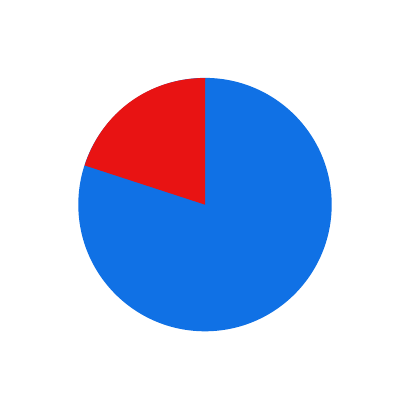
\includegraphics[width=\textwidth]{images/requisiti_tot.png}
    \caption{Schema architetturale del backend}
    \label{fig:Requisiti Totali}
\end{figure}
\newpage
Per quanto riguarda la copertura dei requisiti obbligatori, la copertura rilevata è di 55 su 55
requisiti, arrivando quindi ad un 100\% sul totale

\begin{figure}[H]
    \centering
    
\includegraphics[width=\textwidth]{images/requisiti_o.png}
    \caption{Schema Requisiti Obbligatori}
    \label{fig:Requisiti Obbligatori}
\end{figure}

\newpage

Per quanto riguarda la copertura dei requisiti Desiderabili, la copertura rilevata è di 5 su 12
requisiti, arrivando quindi ad un 41\% sul totale
\begin{figure}[H]
    \centering
    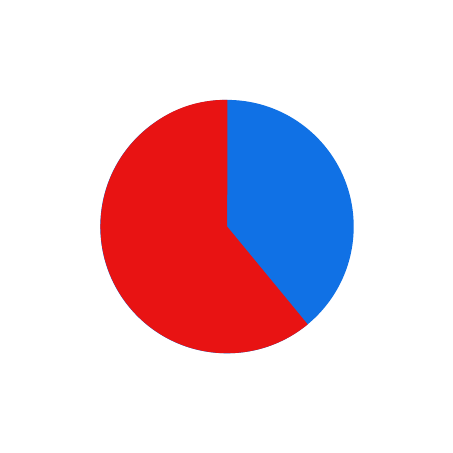
\includegraphics[width=\textwidth]{images/requisiti_d.png}
    \caption{Schema Requisiti Desiderabili}
    \label{fig:Requisiti Desiderabili}
\end{figure}

\newpage

Per quanto riguarda la copertura dei requisiti Desiderabili, la copertura rilevata è di 1 su 9
requisiti, arrivando quindi ad un 11\% sul totale
\begin{figure}[H]
    \centering
    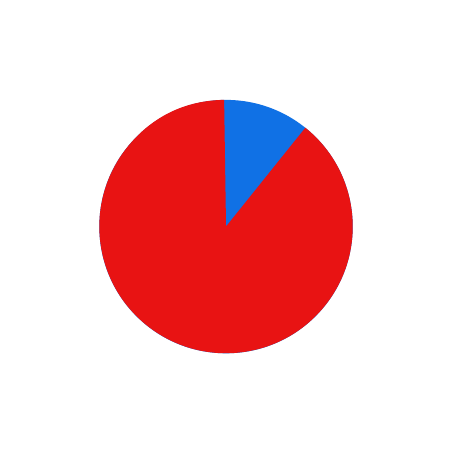
\includegraphics[width=\textwidth]{images/requisiti_op.png}
    \caption{Schema Requisiti Opzionali}
    \label{fig:Requisiti Opzionali}
\end{figure}





